% USE PDFLATEX WITH THIS DOCUMENT. If you wish to use ordinary latex (why?) then convert the figures in figures/ to eps.
\documentclass[masters]{chalmers-thesis}
\usepackage[utf8]{inputenc} % File encoding, you should try to stick to utf8.

\usepackage{amsmath,mathtools} % All your math related needs
\usepackage{microtype} % Magically improves typesetting
\usepackage{biblatex} % Modern package for bibliographies.
\usepackage{listings} % For source code.

\coverfigure{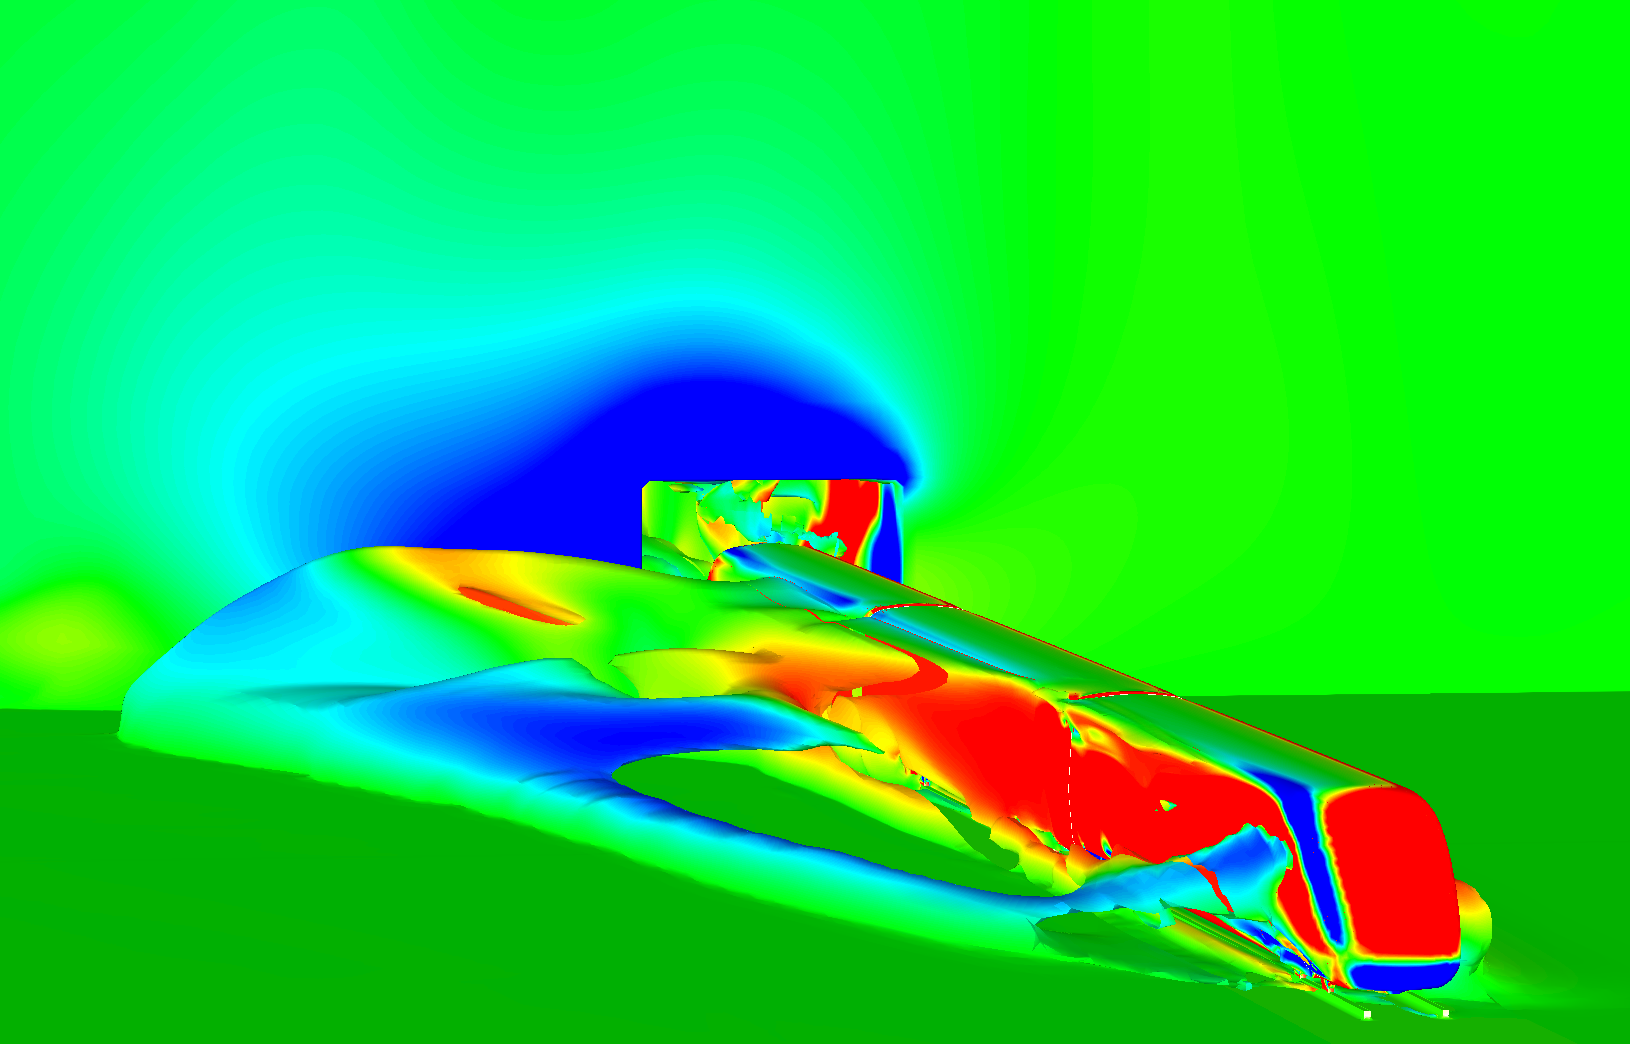
\includegraphics[width=\textwidth,height=0.4\paperheight,keepaspectratio]{figures/COVER_93_iso.png}}
\covercaption{Some explanation}
\title{The Title of Your Thesis which might be very long}
\subtitle{And Perhaps a Subtitle}
\author{Some Author\and Other Author}
\thesis{Master's thesis in Some Programme}
%\thesisin{Master's thesis in Some Programme}
\department{Department of Applied Mechanics}
%\division{Division of Solid Mechanics}
\YYYYNN{2010:37}
%\ISBN{123-21332-13423-123} % Only PhD thesis gets ISBN!
\writtenyear{2010}

\myabstract{Some  short summary asdkasdmkasd asdf sdf fdkfas fd askfm sd fkmasdfm sdkf skmdfksmdfka skd fkasmdf}
\keywords{Some stuff, More stuff, Stuff}

%\bibliography{mybib}

% The following part is automatically generated, go to document start
\newcounter{paper}
\setcounter{paper}{0}
%\renewcommand{\thepaper}{\Alph{paper}}
\newcommand{\paper}[2]{
 \stepcounter{paper}
 \addcontentsline{paper}{toc}{WTF}
 \thispagestyle{empty}
 \begin{flushright}
  {\huge\textbf{Paper \Alph{paper}}}
 \end{flushright}
 \vskip 4em
 {\noindent\Large\textbf{#1}\par}
 \vskip 2em
 \begin{center}
 \begin{minipage}{0.8\textwidth}
   {\noindent\large#2\par}
 \end{minipage}
 \end{center}
 \newpage
}
%\newcommand\section{\@startsection {section}{1}{\z@}%
%                                   {-3.5ex \@plus -1ex \@minus -.2ex}%
%                                   {2.3ex \@plus.2ex}%
%                                   {\normalfont\Large\bfseries}}
%% Writes list of papers as *.lop

\begin{document}
\selectlanguage{english}
\maketitle

\newpage
\tableofcontents
%\phantomsection\addcontentsline{toc}{section}{Sammanfattning}\begin{abstract}\input{SwedishAdstract}\end{abstract}
% or a blank box
%\mbox{}

%\listofpapers
\newpage
\paper{A stude of multiple crack interaction at rolling contact fatigue of rails}{A fricking long citation}
%\
\paper{Assessment of acceleration modeling for fluid-filled porous media subjected to dynamic loading}{cite2}

% Real contents of report starts here
% Splitting it up to several files help when working together.
% Floatbarriers prevent figures from beeing placed into the next chapter.
\section{Introduction}
% \subsection{Background}
Due to the magnitude of the velocity of a high speed train (HST) the flow around it becomes an increasingly important factor. 
The unsteadiness and the different forces and moments that start acting on the train have a big impact on the stability of the train 
and safety and comfort of the passengers. This can probably be countered using damping in the bogies and coupling between the trains.
This is the reason behind this project. To find the forces and moments affecting the train 
and if it's the effects on discomfort and instability can be reduced.
In previous studies of HST instabilities it has either been purely aerodynamic or dynamic with simplified aerodynamic forces.
In this case it is intended to combine them to get an as accurate simulation as possible. 

\subsection{Purpose}
The purpose of this project is to combine two different fields, 
aerodynamics and dynamics, to accurately simulate the HST by
considering all the forces acting on the train in order to get an accurate model.
The goal of this project is to combine the aerodynamic forces that acts on a HST 
with the dynamics on the trains bogie and coupling. 
An interesting final result would be to find how sensitive the dynamics in the train is to varying velocity.

From vehicle dynamics side the focus of the project will be two folds:
\begin{itemize}
\item Create low-order mathematical and computational models for vibration dynamics and stability analysis of HST taking into account 
aerodynamic excitations. 
The models must implement the conventional bogie and conventional car-body coupling functional component mechanical models.
\item Using created models simulate the vibration dynamics and study stability of motion of HST for the two scenarios.
\end{itemize}

\subsection{Limitations}
Two different scenarios were studied. One where two trains meet each other and one where a single train has left a tunnel and is met by a strong wind gust. The model of the train used for the CFD simulations was an ICE2 train. The train consists of two locomotives and one car in the middle making it symmetrical. It has bogies and inter-car gaps. The parameters for the dynamics model were that of a typical HST. For the meeting trains the simulation was carried out at three different velocities, 67 m/s, 70 m/s and 73 m/s, which correspond to 240, 250 and 260 km/h respectively. For the scenario where the train coming out of a tunnel the speed of the train was 70 m/s and the speed of the wind gust was 35 m/s.

\subsection{Approach}
The aerodynamics was simulated with AVL-Fire CFD solver. For the double train, two train models were used with a moving mesh to simulate the two trains meeting each other. For the second scenario with the HST coming out of the tunnel a model of a ICE2 train in a simulated windtunnel with a moving crosswind was used. The forces and moments acting on the each train car on one of the trains were then handed over for the dynamics calculations.

The dynamics were simulated with a low order mathematical model using MATLAB and functional components for bogie and coupling.
The input were the forces and moments calculated from the CFD simulations and the forces acting on the wheels from the rail.
Unknown parameters, such as damping coefficients in the bogie, were decided by minimizing a cost function for comfort and stability.
As a last step, active damping was added to the model.%\FloatBarrier

%\subfile{Theory}\FloatBarrier
%\subfile{Method}\FloatBarrier
%\subfile{Results}\FloatBarrier
%\subfile{Conclusions}
%\subfile{Recommendations}

%\printbibliography

% Appendices
%\subfile{Appendix}

\end{document}

